\documentclass{article}

\usepackage[position]{neurips_2026}

\usepackage[utf8]{inputenc}
\usepackage[T1]{fontenc}
\DeclareUnicodeCharacter{2205}{\ensuremath{\varnothing}}
\usepackage{hyperref}
\usepackage{url}
\usepackage{booktabs}
\usepackage{amsfonts}
\usepackage{amsmath}
\usepackage{amssymb}
\usepackage{nicefrac}
\usepackage{microtype}
\usepackage{xcolor}
\usepackage{graphicx}
\makeatletter
\def\maxwidth{\ifdim\Gin@nat@width>\linewidth\linewidth\else\Gin@nat@width\fi}
\def\maxheight{\ifdim\Gin@nat@height>\textheight\textheight\else\Gin@nat@height\fi}
\makeatother
\setkeys{Gin}{width=\maxwidth,height=\maxheight,keepaspectratio}
\usepackage{longtable}
\usepackage{array}

\providecommand{\tightlist}{%
  \setlength{\itemsep}{0pt}\setlength{\parskip}{0pt}}

\title{Logical and Semantic Guarantees in LLMs Require More Than
Continuous Embeddings}
\author{}

\begin{document}

\maketitle

\begin{abstract}
	This position paper argues that continuous embeddings are insufficient
 as the sole semantic substrate for reliable LLM-based systems.
 Embeddings support similarity, generalization, and retrieval, but they
 do not by themselves define what counts as a valid proposition, a
 category error, a contextual truth, or a recoverable explanation. We
 argue that future AI systems need an additional representational layer:
 locally scoped logical spaces in which linguistic signs are separated
 from logical structure, and propositions are compiled into typed,
 auditable, context-bound coordinates.

 To support this position, we define a representational and operational
 framework for world-local semantic validation. In this framework, each
 local world specifies its own universe of concepts, admissible
 relations, rules of sense, signatures, masks, and denotation functions.
 LLMs or human operators may assist with semantic disambiguation, but
 candidate propositions must pass through symbolic validation before
 being asserted as knowledge. Mathematically, the framework is grounded
 in a contextualized Boolean algebra over typed binary signatures, with
 XOR-based contrasts, Boolean operations for semantic filtering, matrix
 indices over the Boolean semiring, and partition refinements induced by
 discriminative dimensions.

 Our central claim is that hallucination mitigation should not be
 treated only as a retrieval or calibration problem. It should also be
 treated as a representability problem: systems should reject
 propositions that cannot be expressed within the local grammar of
 sense.
\end{abstract}

\hypertarget{introduction}{%
\section{Introduction}\label{introduction}}

The rapid advancement of Large Language Models (LLMs) has demonstrated
an unprecedented capacity for fluent text generation and complex pattern
matching. However, these systems remain plagued by a fundamental
structural unreliability that predates them and is the cause of drift,
unpredictable behaviour and hallucinations, the symbol grounding problem
\citep{harnad1990symbolgrounding}. Current research efforts primarily
address this issue through epistemic improvements, such as
Retrieval-Augmented Generation or Reinforcement Learning from Human
Feedback. We argue, however, that the root of this unreliability is
representational rather than purely informational. The reliance on
continuous vector spaces as the sole substrate for semantic encoding
excels at capturing fuzzy similarities but lacks the discrete primitives
necessary to define the rigorous boundaries of logical sense.
Consequently, current architectures often conflate falsehood with
fundamental inapplicability.

To address this representational gap, this paper argues for the
necessity of a discrete, locally scoped representational layer that
explicitly separates the stochastic nature of linguistic signs from
their underlying deterministic logical structure. Drawing upon the
logical atomism of Ludwig Wittgenstein's Tractatus
Logico-Philosophicus---specifically the premise that the logical
structure of the world is determined by facts rather than isolated
things --- \textbf{we propose a transition from probabilistic distances
to verifiable, algebraic logical coordinates.} Under this framework,
propositions must be evaluated not only by their truth value but by
their state of meaning: \emph{Sinnvoll} (meaningful), \emph{Sinnlos}
(tautological or contradictory), and \emph{Unsinnig} (absurd or
structurally inapplicable).

By treating the validity of assertions as a problem of representability
within a strict grammar of sense, we propose decoupling language
processing into two parallel dimensions. We define a partition of the
world \(W_i\) through a Boolean matrix evaluating Truth \(V_i\) and a
secondary matrix evaluating Sense or applicability \(S_i\). This
separation provides a mathematical mechanism---a ``sense mask''---that
filters out \emph{Unsinnig} (absurd) propositions before they can
perturb the logical evaluation of a system.

Ultimately, instead of attempting to teach models not to lie through
continuous probabilistic weights, this work formally defines an
algebraic architecture that is structurally incapable of representing
nonsense. By mapping structured knowledge into these Boolean matrices,
we present a direct projection between thought and its logical image,
providing a deterministic anchor that could redefine how neural
reasoning and knowledge verification operate in specialized domains.

\hypertarget{state-of-the-art-hallucination-mitigation-and-representational-geometries}{%
\section{State of the Art: Hallucination Mitigation and Representational
Geometries}\label{state-of-the-art-hallucination-mitigation-and-representational-geometries}}

The generation of factually incorrect or logically inconsistent
statements in Large Language Models (LLMs)---commonly referred to as
``hallucinations''---has prompted an extensive body of research. Current
efforts to diagnose and mitigate this structural unreliability can be
categorized into five primary domains: epistemic evaluation, latent
space probing, behavioral interventions, the philosophical defense of
continuous semantic grounding, and neuro-symbolic hybrid architectures.

\textbf{Epistemic Evaluation and Probabilistic Detection} A significant
portion of the literature focuses on auditing LLMs as black-box systems,
attempting to quantify their factual precision post-generation.
Frameworks such as FActScore and HaluEval have been developed to
evaluate factual accuracy at an atomic level
\citep{factscore2023, halueval2023}. Other approaches propose the
detection of hallucinations through ``semantic entropy,'' which measures
the statistical divergence and uncertainty in generated responses to
estimate when a model is confabulating \citep{semantic_entropy2024}.
Complementary work traces these errors to their origin: hallucinations
are not random noise but follow from co-occurrence biases in pretraining
data that continuous representations fail to bound deductively
\citep{mckenna2023}, and from a measurable gap between what models
internally know and what they can reliably verbalize \citep{yin2023}.

\textbf{Internal Representations and Latent Probing} Latent probing
reveals a fundamental discrepancy between internal encoding and
generative behavior. Hallucinations empirically split into two regimes:
\(HK^{-}\), where the model genuinely lacks the knowledge, and
\(HK^{+}\), where the correct answer is encoded in latent activations
but fails to manifest in the output
\citep{orgad2025iclr, simhi2024distinguishing}. Crucially, this
\(HK^{+}\) failure persists even under deterministic decoding (e.g.,
\texttt{argmax}), proving that factual corruption is not merely a
byproduct of stochastic sampling. Instead, the generation of
inconsistencies is inherent to the continuous representational mechanism
itself. The \(HK^{+}\) regime highlights the necessity of a discrete
sense mask: when knowledge is mapped onto a continuous surface lacking
rigid topological boundaries, it remains structurally vulnerable to
corruption. Linear probing indeed recovers emergent truth directions,
though they degrade as logical structure grows complex
\citep{marks2024}; internal-state scores such as EigenScore detect
hallucination risk but only post-hoc \citep{chen2024}; and decoding-time
corrections that contrast final against premature layers (DoLa) mitigate
symptoms without altering the continuous substrate that produced them
\citep{chuang2024}.

\textbf{Behavioral Interventions and Model Collapse} The recursive
ingestion of synthetic, AI-generated content (often termed ``AI slop'')
accelerates a structural degradation known as model collapse
\citep{shumailov2024, kommers2025slop}. To counteract logical drift and
prevent the model from collapsing into statistical loops, the industry
heavily relies on behavioral mitigations such as Reinforcement Learning
from Human Feedback (RLHF) and the implementation of rigid ``state
anchors'' (system instructions) that constrain the model within specific
cognitive frameworks. The same fragility appears during adaptation:
fine-tuning on knowledge unfamiliar to the pretrained model
systematically induces hallucinated factual completions
\citep{gekhman2024, kang2025}, suggesting that continuous weight updates
cannot mark the boundary between acquired knowledge and confabulation.

\textbf{Semantic Grounding and Continuous World Models} From a
philosophical and cognitive perspective, recent literature attempts to
justify the capabilities of LLMs by arguing they are not merely
``stochastic parrots'' without meaning \citep{bender2020}. Authors like
Lyre argue that through self-supervised learning over massive datasets,
LLMs develop ``world models'' encoded within their continuous
representational geometries \citep{lyre2024understanding}. Under this
view, the proximity of activation clusters within the latent space
provides an indirect causal grounding, analogous to Wittgensteinian
``language games'' \citep{lyre2024understanding}. However, while this
perspective defends the statistical extraction of meaning, it accepts
logical confabulations as an inevitable byproduct of a probabilistic
continuous environment, lacking a strict mechanism to enforce rigorous
logical boundaries.

\textbf{Neuro-Symbolic Approaches and Knowledge Graphs} Recognizing the
limits of purely probabilistic reasoning, the field is transitioning
towards neuro-symbolic architectures to implement reliable autonomous
agents \citep{ibrahim2026, ferrone2019}. Significant efforts are being
made to utilize fine-tuned LLMs to translate natural language into
First-Order Logic \citep{vossel2025advancing, liu2025code4logic}, or to
generate verifiable mathematical reasoning \citep{symcode2025}.
Concurrently, there is a strong push toward utilizing LLMs for Knowledge
Graph construction, aiming to map stochastic semantic extractions into
structured, deterministic databases
\citep{choi2025knowledge, bian2025llm}.

\textbf{Why Continuous Spaces Offer No Guarantee of Logical Validity}
The case for discrete primitives rests on three structural observations
about continuous approximation. The first two demonstrate inescapable
mathematical limits of continuous functions approximating discrete
logic, while the third highlights an empirical boundary of current
embedding techniques. First, an indicator of logical validity
\(f(x) \in \{0, 1\}\) is discontinuous at its boundary; smooth
approximators converge to such functions in measure but not uniformly,
and boundary oscillations of the Gibbs type (classically
\(\approx 8.95\%\) of the jump) shrink in width without disappearing,
regardless of scale \citep{hornik1991approximation}. Second, a ReLU
network partitions \(\mathbb{R}^d\) into convex polytopes whose number
grows only polynomially with depth at bounded width
\citep{hanin2017universal}; carving non-convex or discontinuous regions
of semantic invalidity (\emph{Unsinnig}, \(S_i = 0\)) thus demands
exponentially many units, meaning bounded-width networks inescapably
force logical interference at categorical frontiers. Third, as an
empirical limit of current spatial paradigms, probing studies find
factual-discrimination errors lying within the typical channel of the
embedding submanifold, where linear separation performs close to chance
(AUROC \(\approx 0.478\)) \citep{wei2024measuring}. This shows that
current techniques relying on spatial proximity conflate semantic
affinity with factual truth. Deterministic decoding inherits rather than
removes these distortions: \texttt{argmax} over a distorted score
surface is reliably wrong wherever the surface is distorted. A discrete
Boolean primitive (\(S_i \in \{0, 1\}\)) instead imposes a compile-time
boundary \emph{prior} to decoding---a guarantee that continuous
approximation alone does not provide. Formal statements and caveats are
given in Appendix\textasciitilde{}\ref{app:continuous}.

While these current methodologies offer significant advancements, they
fundamentally rely on continuous vector spaces as the ultimate substrate
of evaluation. Whether attempting to mitigate errors via semantic
entropy, probing latent variables, or philosophically defending
continuous world models, these paradigms fail to address the core
dimensional conflict: the conflation between falsehood and fundamental
inapplicability. They lack the discrete primitives necessary to separate
meaningful assertions (\emph{Sinnvoll}) from structural absurdities
(\emph{Unsinnig}) \citep{wittgenstein1922}. To bridge this gap, this
paper proposes transitioning from probabilistic geometries to a discrete
algebraic architecture, separating the evaluation of Truth (\(V_i\))
from a strictly enforced mask of Sense (\(S_i\)), thereby making the
representation of nonsense structurally impossible within bounded
logical spaces (\(W_i\)).

Wittgenstein's Tractatus opens with an interesting phrase: \textbf{the
world is composed of all facts, not things}. We define things as the
atoms that index what can be said (music, theorem, dog, color), and note
that things in the abstract mean nothing; they only acquire meaning
through their relationships. One thing is related to another through
facts (the dog is white, the music is playing, the number adds).
Therefore, what allows the representation of the world and give it a
logical structure is not the empty enumeration of the things that
compose it, but the totality of their relationships.

A proposition is a description of a fact in relation to reality; a fact
that is expressed perceptibly through some medium (sound, written sign,
bits, etc.). A proposition is true or false not based on the fact
itself, but on its relationship with reality. A proposition is
meaningful according to its capacity to demonstrate the truth of the
fact and its capacity to be articulated within a logical framework.
Based on its state of meaning, a proposition can be distinguished into
three states.

\begin{itemize}
\item
  \emph{Sinnvoll}: propositions that are meaningful and capable of
  representing a possible situation in the world. For example, in Spain
  the climate is warm, Beethoven wrote his Ninth Symphony,
  electromagnetic phenomena can be described by Maxwell's four
  elementary equations, etc.
\item
  \emph{Sinnlos}: propositions that say nothing about the world but
  legitimately belong to logical symbolism, such as tautologies and
  contradictions. For example, \emph{goes up upwards}, \emph{a person is
  a human}, Schrödinger's cat is both dead and alive at the same time.
\item
  \emph{Unsinnig}: formulations without logical meaning, where the
  symbols have not been given a significant function within the system;
  in other words, absurd propositions. \emph{The dog rides}, \emph{the
  reason for unreason}, \emph{p = \textasciitilde p}, etc.
\end{itemize}

A sign is the perceptible medium that allows the mapping and
transmission of a fact, an object, or their relationships. It can be a
sound signal, a quality of a sound signal, written text, an image,
music, a theorem, a code, among many others. The sign is not the fact
itself, but rather a mapping of the fact to that which can be expressed.
A fact can be expressed in many signs; the dog is friendly, the canine
is reliable, and the dog is man's best friend all express the closeness
of both specimens; 3 in Arabic notation, 00000011 in binary, and drei in
German designate the same numerical quantity. Similarly, a sign can
represent different symbols; in English, gift is an object given for
free, while in German it means poison; the act of nodding one's head
vertically is commonly accepted as an affirmative gesture, but in
Bulgaria it means no.

A symbol is a sign and a structure within a logical space, used within a
context; that is, within a sufficiently defined partition of the world.
A name is a reference to this logical structure, that is, a mapping
between sign and symbol, sufficiently determined by the context to
distinguish it from other symbols.

\hypertarget{proposed-representation}{%
\section{Proposed representation}\label{proposed-representation}}

Consider the logical structure of a partition of the world \(W_i\) by
the following symbolic set:

\begin{enumerate}
\def\labelenumi{\arabic{enumi}.}
\tightlist
\item
  A context, that is, a partition over the world \(W\) that limits what
  belongs into \(W_i\).
\item
  A logical space \(L_i\) that describes the admissible mapping
  coordinates, for example objects and their properties.
\item
  A Boolean matrix \(V_i\) that describes all the relationships that map
  the facts in relation to their truth.
\item
  A Boolean matrix \(S_i\) that describes all the relationships that map
  the facts in relation to their meaning; that is, their applicability
  within the logical space.
\end{enumerate}

\begin{figure}
\centering
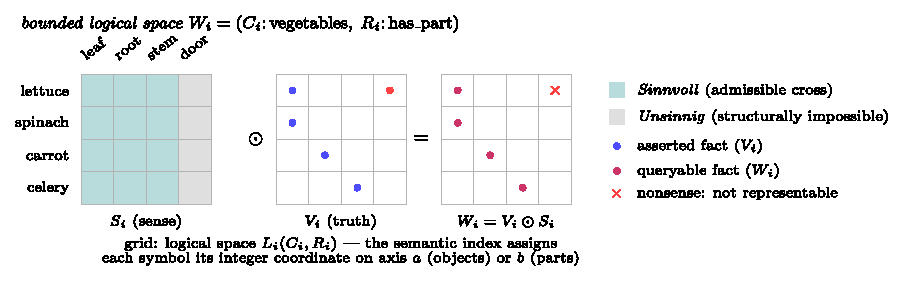
\includegraphics[width=1\textwidth,height=\textheight]{../figures/fig_layers.pdf}
\caption{A context \(W_i=(C_i,R_i)\) instantiates two boolean layers
over the same \(L_i\) grid: the sense mask \(S_i\) (admissible crosses)
and the truth layer \(V_i\) (asserted facts). Queries see only the
operative projection \(W_i^{*}=V_i\odot S_i\): an injected fact outside
the mask is structurally invisible. \label{fig:layers}}
\end{figure}

Then, we can define \(W_i\) as the boolean AND operation between \(V_i\)
and \(S_i\) (see Figure\textasciitilde{}\ref{fig:layers}). Consider this
small example;

\begin{longtable}[]{@{}llrrrr@{}}
\caption{Matrix \(W_i\) mapping objects to their
properties.}\tabularnewline
\toprule
& vegetable & food & leaf & root & stem \\
\midrule
\endfirsthead
\toprule
& vegetable & food & leaf & root & stem \\
\midrule
\endhead
lettuce & 1 & 1 & 1 & 0 & 0 \\
spinach & 1 & 1 & 1 & 0 & 0 \\
carrot & 1 & 1 & 0 & 1 & 0 \\
celery & 1 & 1 & 0 & 0 & 1 \\
\bottomrule
\end{longtable}

It is important to note that within this logical space, the properties
``vegetable'' and ``food'' are true for all objects containing our
\(W_i\), that is, they are tautological under the Tractatus definition
and are therefore meaningless (\emph{sinnlos}). We begin by removing
them to facilitate further analysis. \(W^{T}_i\), the transversal of
this would essentially be an index of properties and which object they
belong to.

\begin{longtable}[]{@{}lrrrr@{}}
\caption{Matrix \(W^{T}_i\), the transversal index of properties and
their corresponding objects.}\tabularnewline
\toprule
& lettuce & spinach & carrot & celery \\
\midrule
\endfirsthead
\toprule
& lettuce & spinach & carrot & celery \\
\midrule
\endhead
leaf & 1 & 1 & 0 & 0 \\
root & 0 & 0 & 1 & 0 \\
stem & 0 & 0 & 0 & 1 \\
\bottomrule
\end{longtable}

If we designate a Boolean semiring AND/OR over this space, we can verify
some useful results.

\begin{itemize}
\tightlist
\item
  If we perform matrix multiplication of \(W^T_i \otimes W_i\), we can
  obtain a map of property co-occurrences.
\item
  The matrix \(W\) serves as an indexing space, meaning we can take a
  one-hot-encoded vector of properties \(v_q\) that denotes the objects
  we want to find. And by vector multiplication \(W_i \otimes v_q\) find
  those vegetables that meet these properties.
\end{itemize}

Returning to the categories of sense defined in Section 2, the logical
restrictions of this system become clear. \emph{Sinnlos} denotes
computable operations that yield no distinguishing information: either
tautologies (e.g., searching for ``food'' returns all objects) or
contradictions (e.g., searching for ``leaf'' and ``stem''
simultaneously). Conversely, \emph{Unsinnig} corresponds to operations
that are structurally inexpressible because no coordinate exists in
\(L_i\) (such as asking for a vegetable's ``doors'' or an unmapped
property like ``sweet taste'').

Up to this point, the proposed system aligns with standard Boolean logic
without offering anything new to the fundamental works of logic and
computation. However, its true utility emerges once we introduce
indexability and unambiguity, as restrictions that allow turning this
into a kind of logical truth machine.

We first address its extensibility. Extending \(W_i\) to contain new
facts is a straightforward operation. If the fact has a defined
coordinate (object, property) that is mappable to the current \(L_i\),
the mechanism is to find the coordinate and set its value to true.
Otherwise, the operation will require adding a new object or property to
the coordinates and check its truthfulness \(W_i\) and sense \(S_i\) for
every other proposition that the dimensional addition generates.

Regarding ambiguity in \(W_i\), the proposed system allows the detection
of it through an elementary algebraic operation.

\begin{itemize}
\item
  \(W_i \otimes W^T_i\) yields a matrix of objects against objects,
  containing all the facts that denote some truthfulness in the map.
  Note that, in this case, since we are interested only in the objects
  that share some property in reality, the sense layer \(S_i\) can
  simply be ignored. Furthermore, the intersection of anything with ∅
  can simply be considered 0.
\item
  \((W_i \otimes W^T_i) - \mathbb{I}\) clears the diagonal, which
  contains only tautological results.
\item
  Finally, by dimensionally collapsing this matrix by multiplying it by
  a vector of ones, we can detect those objects that are colliding in
  some property in \(W_i\).
\end{itemize}

Then, to disambiguate these objects, we introduce a new property to
\(L_i\) that will allow differentiating them. In our case, since the
collapse dimension is a leaf, the easiest thing to do is to add
inherited properties to it, for example, rough and smooth.

\begin{longtable}[]{@{}lrrrrr@{}}
\caption{Extended matrix with inherited properties and sense mask
(\(\emptyset\)) for invalid coordinates.}\tabularnewline
\toprule
& leaf & root & stem & (leaf) rough & (leaf) smooth \\
\midrule
\endfirsthead
\toprule
& leaf & root & stem & (leaf) rough & (leaf) smooth \\
\midrule
\endhead
lettuce & 1 & 0 & 0 & 0 & 1 \\
spinach & 1 & 0 & 0 & 1 & 0 \\
carrot & 0 & 1 & 0 & Ø & Ø \\
celery & 0 & 0 & 1 & Ø & Ø \\
\bottomrule
\end{longtable}

Another detail becomes apparent: if we partition by lettuce and spinach
over leaf-related properties, ``leaf'' becomes a tautological
(\emph{sinnlos}) property. However, for carrot and celery, these newly
introduced leaf properties are \emph{unsinnig}: any truth value computed
for them is structurally meaningless. The solution can be approached in
two ways:

\begin{itemize}
\item
  Use a sense mask \(S_i\) around the facts that are indexable by these
  objects and properties, setting the result to 0 for every possible
  case if querying about truth.
\item
  Create another matrix \(W_i'\) that indexes only leafy vegetables.
  Then, the operation to search for vegetables by the property about
  their leaves becomes \(W_i \otimes p'_i \otimes W'_i \otimes p'_i\).
\end{itemize}

This yields some interesting results:

\begin{itemize}
\tightlist
\item
  \(W_i\) is basically a hierarchical routing space that partitions
  \(W_i \cup W'_i\), in other words, a context index over a tensorial
  logic space where we can identify objects by their properties without
  the need to use \(S_i\).
\item
  The tensorial expansion and collapsing are reversible:
  \(S( W_i \cup W'_i)\) can be recovered by filling the facts that the
  properties of \(L'_i\) do not map in \(L_i\) with Ø.
\item
  The process is infinitely recursive, enabling unions, intersections
  and every other set operations that a boolean ring allows. And as long
  as we correctly permute the dimensions, we can reorganize the
  tensorial routes as we want.
\item
  The introduction of hierarchies of contexts enables the use of this
  logic as a tree search index. Or, to treat a tree search index as a
  combination of truth and sense matrices.
\item
  In the proposed example, we worked with an \(L_i\) that mapped objects
  to properties, but \(L\) contains every relation expressible with
  boolean logic. State machines, s-expressions, if-else flows, among
  others, are just instances of what can be computed with the
  combination of sense and logic.
\item
  Finally, by the usage of these results, we can obtain partitions of
  \(S\), as a set of algebraically computable logical grammar rules for
  determined contexts.
\end{itemize}

In Wittgenstein's words, we have defined a direct projection between
thought and its logical image, represented in bits and operable through
Boolean logic.

\hypertarget{discussion}{%
\section{Discussion}\label{discussion}}

The task of processing text and extracting semantic logic from it has no
novelty. Mapping facts and relations to matrices is a technique with a
long history in computing, as seen in what is commonly known as lookup
tables. Also, handling non-informative bits in logical operations using
the null state Ø is a standard practice in digital system design.
Moreover, handling different ordered tables as relational databases has
its own language and rules in SQL. However, it is the
philosophical-logical substrate that Wittgenstein's Tractatus provides,
which makes this approach useful.

\hypertarget{relationship-with-language}{%
\subsection{Relationship with
Language}\label{relationship-with-language}}

While existing neuro-symbolic and parsing works often translate language
into logical forms (as reviewed in Section 1), they generally fail to
explicitly formalize the difference between truth, applicability/sense,
and algebraic disambiguation of the sign. Furthermore, no current
framework appears to use the triad of context, logic, and sense as
extractable, operable properties across document domains.

Two families of neighboring work clarify what is new here. Retrieval
pipelines and knowledge graphs capture \emph{semantic
co-occurrence}---which entities and phrases appear together---but not
\emph{logical paths}: a KG edge records that two nodes are related, with
no category for combinations that are ill-formed in the first place, and
recent benchmarks show LLM-based graph construction still produces
unfaithful structures \citep{sansford2024grapheval}. Our proposal is
closer in spirit to description logics and causal networks (KL-ONE,
CLASSIC, conceptual graphs), which do constrain what can be consistently
asserted \citep{brachman1990, lehmann1992, sowa1991, kruse2022causal};
indeed, OWL ontologies enter our framework directly as input to the
ingestion pathway. What we add to that lineage is an explicit, operable
category of semantic inapplicability: sense is stored as a matrix layer
\(S_i\), and \emph{Unsinnig} is rejected at compile time inside the
substrate. Crucially, whereas traditional OWL ontologies and KGs rely on
iterative graph traversals (\(\mathcal{O}(V+E)\)) or external deductive
theorem provers to diagnose consistency after the fact, our framework
evaluates both transitive closure and semantic applicability via dense
bitwise matrix multiplication. This pushes logical verification down to
\(\mathcal{O}(1)\) operations on native silicon registers, bypassing the
bottleneck of traditional logical inference.

An interesting first approach to semantics in language is that the
formalization proposed in this work would allow the generation of
document families where the shared logic can be audited not only by its
degrees of truthfulness but also by its states of sense. In other words,
the use of the proposed tools would enable the creation of curated
knowledge graphs, prepared to operate on particular domains with
explicit limits on the context they admit. Furthermore, the proposal
presented in this work explicitly rejects the possibility of a complete
mapping of universal and computable logical universes. The case of the
UNL project, \emph{Universal Network Language}, from the United Nations
Institute for Advanced Studies, demonstrates the difficulty of
encompassing a complete language that maintains both logical coherence
and extensibility.

An important limitation to note at this point is that, as the treatise
anticipates, the distinction between the concept represented in a
knowledge graph and the textual sign that denotes it (token or word)
does not belong to the realm of formal logic. The universe of possible
contexts involved between natural language and its underlying logic
makes the exact calculation of all of them intractable. In other words,
there is a real possibility that the mapping of words to symbols is
unequivocally stochastic in nature. Fortunately, recent advances in
natural language processing models, and especially in neural network
language models such as LLMs, make this task much more manageable than
it was a few years ago.

Furthermore, a little-explored feature of language is that, by defining
a closed set of signs and facts, the mapping of those signs and facts to
language can shift from a stochastic process to a deterministic logical
process, determined by two separate logical processes. First, structured
knowledge, as presented in the previous section, and second, a
``representation surface'' layer, determined by the document structure
and the grammar of the language to be represented. The combination of
these would allow the representation of any type of ``structured
language'' document by the combination of abstract syntax trees and the
Boolean algebra described above. It is worth noting that while this type
of representation would have serious problems representing certain
regional dialects or more artistic and creative documents like poetry,
it would be very well suited to other types of documents that, by
nature, tend to be more structured, such as reports, dictionaries,
technical documentation, or computer code.

Two design notions make this operational at scale: \emph{closed
representations}, within which sense is near-trivial and violations
emerge only at structurally inadmissible context crossings, and the
\emph{omnirepresentation}, a block-matrix form exposing contexts,
routing and facts jointly to stochastic models. The formal construction,
the ingestion pathway, the self-optimization algorithm and the
sense-mask integration are given in
Appendix\textasciitilde{}\ref{app:repr}.

\hypertarget{relationship-with-llm}{%
\subsection{Relationship with LLM}\label{relationship-with-llm}}

An interesting approach to how this proposal relates to the burgeoning
field of neural network language models is the role that the sense mask
\(S\) can play across both training and inference pipelines. Given a
sufficiently large knowledge base, built on the same body of documents
used for training, obtaining a sense mask from the input text at train
time would allow early control over which information is more or less
important through sense detection. Similarly, sense detection in the
generated text would enable a new, automated form of text loss
detection, opening a new dimension within reinforcement learning,
synthetic dataset generation, and even early prevention of outputs the
model might generate during inference.

On the other hand, by introducing context as a limit to the family of
texts we can unite in a logically \emph{sinnvoll} universe, we are
providing accurate tools for curating datasets, while also facilitating
the training of models that function not as universal language machines,
but as specialist machines for specific domains (something sought after
today by SMLs). The effect of this would be greatly amplified if, in
addition to the direct loss in text processing and generation, we
introduced a logical loss in the intermediate layers, thus separating
the processing of language as a sign, with all its inherent imprecisions
and ``grammatical sugar,'' from symbolic representation and sense.

This last point aligns directly with what LeCun and colleagues have been
proposing in JEPA and H-JEPA
\citep{lecun2022path, dawid2024latent, assran2023ijepa}. In their case,
decoupling the abstract representation of the sign ``token by token'' is
being attempted through a combination of two things: the use of scalar
energy to measure compatibility between input and output, and the use of
multidomain embeddings. In our case, this could be decoupled into two
independent levels: the data as a sign and the representation of its
logic and sense.

Finally, one might ask whether a logic machine with sufficient
``knowledge'' could replace what LLMs can do today. The answer is most
likely no. The generalization capacity of a machine based solely on
facts and logical operations on them is, by definition, null. While it
is possible to represent a significant number of tasks and their
solutions through the appropriate combination of algorithms and fact and
context trees, a machine built this way will always struggle to handle
novel situations if it lacks the ``creative'' capacity provided by
stochastic algorithms. However, given that current stochastic algorithms
are based on digital systems that also operate on boolean logic at the
bit level, it is worth asking how stochastic the training and operation
of the neural networks that make up LLMs really are.

\hypertarget{conclusion}{%
\section{Conclusion}\label{conclusion}}

In conclusion, this paper has presented a formal framework to bridge the
relationship between natural language and structured knowledge. By
transitioning from continuous vector spaces---which inherently conflate
the probability of the stochastic sign with its logical validity---to a
discrete algebraic system grounded in Wittgenstein's categories of
sense, we have proposed an architecture capable of evaluating
information across two parallel dimensions: truth (\(V_i\)) and sense or
applicability (\(S_i\)). Through this ``sense mask,'' we demonstrate
that it is mathematically possible to project a direct logical image of
thought operated entirely through Boolean algebra, isolating and
neutralizing absurd propositions (\emph{Unsinnig}) before they can
perturb the system's reasoning.

While the body of this work has focused on establishing the theoretical
and algebraic foundations of this model without presenting empirical
evaluation metrics, the proposed framework is not purely hypothetical.
Currently, a functional implementation exists that validates this
architecture by combining the text-processing capabilities of Large
Language Models (LLMs) with the matrix algebra described herein. This
implementation is actively used for logical extraction and the creation
of curated knowledge graphs, where the information extracted by LLMs is
rigorously audited not only by its degrees of truth but also by its
states of meaning within strictly bounded contexts (\(W_i\)).

Future work will focus on closing this computational loop. Having
demonstrated that LLMs can be utilized to map language onto these
deterministic knowledge bases, the next step is to use this
algebraically structured knowledge to generate and train new neural
architectures. This includes integrating sense masks directly into
attention mechanisms to penalize automated text loss, as well as the
curation of highly precise synthetic datasets. The ultimate goal is to
leverage this symbolic logic to train ``specialist machines'' for
specific domains; models that function not as universal stochastic
language generators, but as systems inherently anchored to a grammar of
sense where logical hallucinations are, by design, structurally
impossible to express.

\bibliographystyle{plainnat}
\bibliography{references.bib}

\hypertarget{appendix}{%
\section{Appendix}\label{appendix}}

\hypertarget{on-the-geometric-origin-of-hallucinations}{%
\subsection{\texorpdfstring{On the Geometric Origin of Hallucinations
\label{app:hallucinations}}{On the Geometric Origin of Hallucinations }}\label{on-the-geometric-origin-of-hallucinations}}

To understand why continuous semantic spaces struggle with factual
accuracy, we can look at how the literature maps hallucinations to their
geometric origins in the embedding space \(\mathbb{R}^d\). Recent
evaluation frameworks classify structural generation errors into three
geometric types based on their spatial behavior within semantic
submanifolds \citep{wei2024measuring, sansford2024grapheval}:

\textbf{Type I: Infidelity (Contextual Deviation)} This occurs when the
generation strays from the provided context or the required semantic
channel. Geometrically, the output vector drifts away from the target
submanifold. Because this represents a significant spatial deviation,
Type I errors are readily detectable using standard continuous distance
metrics (e.g., cosine distance) or entropy measurements, typically
yielding an AUROC \(> 0.80\) \citep{wei2024measuring}.

\textbf{Type II: Confabulation (Domain Mismatch)} This happens when the
model hallucinates a completely unrelated topic or bizarre assertion.
Geometrically, these outputs fall far outside the expected distribution.
Like Type I errors, Type II errors are easily flagged as
out-of-distribution anomalies using continuous metrics (AUROC
\(> 0.75\)).

\textbf{Type III: Factual Error (In-Channel Falsehood)} This is the most
pernicious error: the model generates an incorrect fact while staying
perfectly within the correct conceptual framework. Because semantically
related truths and falsehoods share the same geometrical neighborhood,
Type III errors reside \emph{inside} the typical channel of the
representation. As demonstrated by Wei et al., linear discrimination for
these in-channel errors performs close to chance (AUROC
\(\approx 0.478\)) \citep{wei2024measuring}.

The geometric detectability of Types I and II often creates the
``Self-Correction Illusion'' \citep{symcode2025}---the belief that
scaling or better continuous monitoring will eventually solve all
hallucinations. However, the AUROC barrier of Type III errors
demonstrates a structural limit of current spatial paradigms: continuous
distance encodes statistical co-occurrence, not factual truth. Resolving
Type III errors therefore requires stepping outside the continuous
spatial paradigm and introducing a discrete verification step.

\hypertarget{on-the-limits-of-continuous-approximation}{%
\subsection{\texorpdfstring{On the Limits of Continuous Approximation
\label{app:continuous}}{On the Limits of Continuous Approximation }}\label{on-the-limits-of-continuous-approximation}}

This appendix details the three observations from Section 2. The first
two establish inescapable mathematical limits when using continuous
functions and bounded-width architectures to approximate discrete logic.
The third observation highlights an empirical failure specific to
current embedding methodologies rather than an absolute impossibility
result for neural networks.

\hypertarget{indicator-boundaries-and-inescapable-oscillation}{%
\subsubsection{Indicator boundaries and inescapable
oscillation}\label{indicator-boundaries-and-inescapable-oscillation}}

Let \(f: \mathbb{R}^d \to \{0,1\}\) indicate logical validity,
discontinuous at the boundary of its support. Universal approximation
results \citep{hornik1991approximation} guarantee convergence in \(L^1\)
/ in measure: the \emph{mass} of the error region can be made
arbitrarily small. Convergence is not uniform, however: near a jump, any
smooth or piecewise-smooth approximator exhibits a transition band with
overshoot---the Gibbs phenomenon, whose classical overshoot is
\(\approx 8.95\%\) of the jump magnitude. Narrowing the band requires
steeper activations and more units, but the band does not vanish with
more data or training; it is a fundamental mathematical property of
approximating a jump with continuous functions. In semantic terms, this
inescapable limit means there is always a region where \emph{Unsinn}
receives an intermediate score instead of a strict exclusion.

\hypertarget{polytope-tiling-at-bounded-width}{%
\subsubsection{Polytope tiling at bounded
width}\label{polytope-tiling-at-bounded-width}}

A ReLU network is piecewise affine: each neuron's activation boundary is
a hyperplane, and their arrangement partitions \(\mathbb{R}^d\) into
convex polytopes on which the network is linear. For width \(w \le d\)
and depth \(L\), the number of regions is bounded by

\[\mathcal{N}(w, L) \le \sum_{j=0}^{d} \binom{wL}{j},\]

which grows polynomially in \(L\) \citep{hanin2017universal}. Sense
boundaries, by contrast, are typically non-convex and disconnected: type
constraints over symbols combine combinatorially, so the set of
\emph{sinnvoll} propositions scatters across many disconnected regions.
Tiling such a set with convex cells requires a number of regions
exponential in the number of constraints. While unbounded networks could
theoretically escape this limit, any bounded-width network inevitably
suffers from a structural deficit. This inescapably forces logical
interference at categorical frontiers, making it an absolute limit
within practical architectural constraints.

\hypertarget{the-soft-boundary-of-current-embedding-techniques}{%
\subsubsection{The soft boundary of current embedding
techniques}\label{the-soft-boundary-of-current-embedding-techniques}}

If factual errors were outliers in embedding space, post-hoc detection
would be easy. However, probing studies find that factual
errors---incorrect facts within the correct conceptual
framework---reside inside the typical channel of the representation.
Here, linear discrimination performs close to chance (AUROC
\(\approx 0.478\)) \citep{wei2024measuring}. Unlike the first two
mathematical limits, this represents a soft boundary of current spatial
methodologies: distance metrics in embedding spaces encode statistical
co-occurrence, not factual correspondence. Because semantically related
truths and falsehoods share the same geometrical neighborhood, current
continuous scalar reads fail to reliably separate valid from invalid
generations---motivating a check that lives outside the continuous
substrate.

\hypertarget{on-deterministic-decoding}{%
\subsubsection{On deterministic
decoding}\label{on-deterministic-decoding}}

\texttt{argmax} is a deterministic function of the score surface:
wherever the surface is distorted, decoding is wrong
\emph{reproducibly}, with no sampling randomness to blame. This cuts
both ways---stochastic decoding is not the culprit either; both inherit
the substrate. The design conclusion is that the boundary must be
imposed \emph{before} decoding, at compile time, where a stored Boolean
matrix \(S_i\) provides an exact check in \(O(1)\) per step instead of
an approximate one distributed across the network.

\hypertarget{closed-representations-omnirepresentation-and-the-operational-pathway}{%
\subsection{\texorpdfstring{Closed Representations, Omnirepresentation,
and the Operational Pathway
\label{app:repr}}{Closed Representations, Omnirepresentation, and the Operational Pathway }}\label{closed-representations-omnirepresentation-and-the-operational-pathway}}

\hypertarget{formal-backbone-logical-form-as-a-matrix}{%
\subsubsection{Formal backbone: logical form as a
matrix}\label{formal-backbone-logical-form-as-a-matrix}}

In the Tractarian reading that structures our substrate, logical
form---``the possibility of structure'' (2.033)---is instantiated as the
syntax matrix \(S_i\): an adjacency operator over the object layer
\(V_i\) that restricts which combinations are structurally possible
\emph{before} any truth evaluation,
\(\text{PossibleStructure} = \sigma(V_i \times S_i)\). Atomic facts are
minterms---exhaustive boolean conjunctions over the base variables,
stored operatively as (concept, dimension, discriminative value) tuples,
e.g., \texttt{(lettuce,\ edible\_part,\ leaf)}---so the world is the
tensor region of active minterms. A proposition has \emph{sense} (Sinn)
iff it partitions minterm space properly (neither the all-ones tautology
nor the all-zeros contradiction; those are \emph{sinnlos}, senseless);
it is \emph{unsinnig} when it falls outside the span of \(S_i\)
altogether---a type violation, rejected at compilation, not a falsehood.
Figure\textasciitilde{}\ref{fig:signsymbol} pictures the sign/symbol
periphery (\S2) and the semantic index \(L_i(C_i,R_i)\) that assigns
integer coordinates; the two boolean layers \(S_i\), \(V_i\) and their
queryable product are Figure\textasciitilde{}\ref{fig:layers} (\S1).

\begin{figure}
\centering
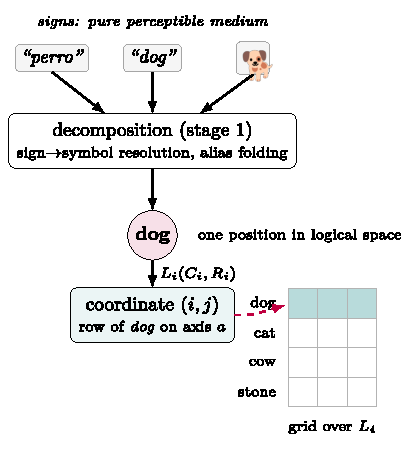
\includegraphics[width=0.55\textwidth,height=\textheight]{../figures/fig_sign_symbol.pdf}
\caption{From signs to coordinates. Perceptible signs---the word
\emph{perro}, the word \emph{dog}, a dog pictogram---converge through
the decomposition stage (sign\(\to\)symbol resolution and alias folding)
onto a single symbol: one position in logical space, independent of
language. The semantic index \(L_i(C_i,R_i)\) then fixes its integer
coordinate on an axis of the context grid. The system computes over
coordinates, never over signs. \label{fig:signsymbol}}
\end{figure}

\hypertarget{closed-representations}{%
\subsubsection{Closed representations}\label{closed-representations}}

A context \(w_i\) is \emph{closed} when its axes are typed locally:
objects on each axis belong to the same local type and the context's
rules range only over its own symbols. Within a closed context \(S_i\)
is near-trivial---almost all coordinates are admissible, and the real
question is factual
(\(V_i \in \{\text{true}, \text{false}, \emptyset\}\)). Sense structure
becomes necessary exactly when contexts are \emph{crossed}: objects of
one domain with properties of another. Crossings then fall into three
classes---\emph{sinnvoll} (admissible), \emph{don't care} (outside the
subcontext, not evaluated), and \emph{unsinnig} (violates categorial
structure). A type layer \(T_i\) validates that relational signatures
align before any composition \(W_1 \otimes p \otimes W_2\) is allowed,
so \(S_i=0\) cannot arise from accidental context incongruence: it is
structurally emergent, and therefore derivable from the schemas rather
than hand-listed.

\hypertarget{the-omnirepresentation}{%
\subsubsection{The omnirepresentation}\label{the-omnirepresentation}}

Composition is realized in a single block matrix, the
\emph{omnirepresentation}, laid out in four quadrants: the top-left
\(m \times m\) quadrant (\(WC_i\)) routes and activates contexts; the
top-right and bottom-left \(m \times n\) quadrants hold don't-care
membership blocks routing which facts belong to which context---this
routing \emph{is} the sense mask at composition level; and the
bottom-right \(n \times n\) quadrant holds the empirical truth matrix.
Globally, knowledge exists as one canonical hypertensor
\(N \times |R| \times N\); operationally it materializes as a graph of
dense 2D sub-matrices extracted by tensorial projection, alternating
between the flat empirical view (\(V_i, S_i\)) and the hierarchical
tensorial view in which global attributes are promoted to routing
hyperdimensions. This form provides the flexibility the internal ``pure
matrix'' engine deliberately lacks: \(S_i\) can be applied over
\emph{unions of contexts} by activating several routing entries; the
whole structure is a flat, ingestible view a stochastic model can read
and write (massive I/O interface for LLMs); and any external
computation---an LLM's candidate facts, a matrix calculation over
embeddings---can be checked against the same blocks without format
conversion.

\hypertarget{operational-ingestion-pathway}{%
\subsubsection{\texorpdfstring{Operational ingestion pathway
\label{app:ingestion}}{Operational ingestion pathway }}\label{operational-ingestion-pathway}}

From natural language to an audited proposition, four stages:

\begin{enumerate}
\def\labelenumi{\arabic{enumi}.}
\tightlist
\item
  \textbf{Decomposition into standard form.} The utterance is decomposed
  into its meaning plus syntactic sugar, and the meaning is expressed in
  a standardized representation---S-expressions, RDF/Turtle, or OWL. We
  propose small LLMs as surface decomposers: they absorb sign
  variability (including sign-to-symbol resolution and alias folding)
  but make no logical decisions.
\item
  \textbf{Reduction to candidate propositions.} The standard form is
  lowered to homogeneous candidate propositions
  \texttt{(R\ a\ b)}---e.g., \texttt{(sound\ dog\ barks)},
  \texttt{(sound\ cat\ meows)}. Nothing here is asserted yet; candidates
  have no truth status.
\item
  \textbf{Two-step sense check.} (a) \emph{Context indexing:} the
  candidate is routed to the context(s) that index its cross; if no
  context admits the (domain, relation) combination, the candidate is
  rejected as \emph{Unsinnig}---absurdity is avoided by construction,
  before any truth evaluation. (b) \emph{Contradiction check:}
  admissible candidates are checked against the existing facts \(V_i\)
  of their context; a conflict with what is already asserted yields an
  explicit contradiction signal rather than silent overwrite.
\item
  \textbf{Matrix computation.} Only candidates passing both checks
  update or consult \(V_i\); inference proceeds by boolean matrix
  multiplication and bitwise dimensional collapse, yielding
  \(W_i^{*} = V_i \odot S_i\).
\end{enumerate}

\emph{Worked example.} \emph{``The edible part of lettuce is the leaf''}
is decomposed and reduced to the candidate
\texttt{(edible\_part\ lettuce\ leaf)}. Context indexing routes it to
the food context, which admits the cross (3a passes); no conflicting
fact exists in \(V_i\) (3b passes); the tuple is asserted and
participates in closure. By contrast,
\texttt{(has\_color\ electron\ red)} fails step 3a in any closed
physical-entity context---the (particle, color) cross violates
categorial structure---and is rejected as \emph{unsinnig} before a truth
value can attach. Finally, \texttt{(sound\ cat\ barks)} submitted after
\texttt{(sound\ cat\ meows)} was asserted passes 3a (the cross is
admissible) but fails 3b: the system reports an explicit contradiction
instead of silently overwriting the earlier fact.

\hypertarget{self-optimization-er-minimization-and-the-hierarchical-tensor}{%
\subsubsection{\texorpdfstring{Self-optimization: \(E(R)\) minimization
and the hierarchical tensor
\label{app:er}}{Self-optimization: E(R) minimization and the hierarchical tensor }}\label{self-optimization-er-minimization-and-the-hierarchical-tensor}}

Construction is not manual \(\mathcal{O}(N^2)\)---and a purely diagonal
index is provably suboptimal, collapsing asymptotically to
\(E(R) \to 0.5\). Two deterministic mechanisms keep the substrate
compact:

\begin{itemize}
\tightlist
\item
  \textbf{Information-energy minimization.} The engine scores each
  logical space with \(E(R) = \frac{1}{4}(c + i + o + d)\)---sense
  density, facticity, observed-fact rate, and discriminative power---and
  applies mutations only when \(\Delta E(R) > 0\): constant
  (tautological) columns are promoted to tensor gates, contexts whose
  sense density drops are split into clean sub-contexts, and collisions
  in \(W_i \otimes W_i^{T} - \mathbb{I}\) trigger injection of a minimal
  separating dimension. This is a deterministic analogue of training,
  run as maintenance after bulk ingestion.
\item
  \textbf{Hierarchical tensor construction.} A common attribute (e.g.,
  \texttt{is\_vegetal}) becomes a partition dimension \(C_k\); entities
  are factored into child sub-tensors linked by routing projections
  \(WC_k\), and multi-hop queries navigate
  \(P = WC_1 \otimes \dots \otimes WC_k\), reducing spatial complexity
  toward \(\mathcal{O}(N \log N)\).
\end{itemize}

\hypertarget{sense-mask-integration-with-stochastic-models}{%
\subsubsection{\texorpdfstring{Sense-mask integration with stochastic
models
\label{app:mask}}{Sense-mask integration with stochastic models }}\label{sense-mask-integration-with-stochastic-models}}

The mask enters at two levels. \emph{At runtime}, the engine rejects
deterministically at three checkpoints---\texttt{ingest},
\texttt{check}, \texttt{assert}: a proposition with \(S_i = 0\) never
enters the veritative system, and the caller receives an explicit
\texttt{reject\ (unsinnig)} signal; generation whose continuations all
fail is halted and reported as unanswerable in the context. \emph{Inside
a Transformer} (proposed integration), the mask is injected additively
into attention,

\[\text{Attention}(Q, K, V) = \text{Softmax}\Big(\frac{QK^T}{\sqrt{d_k}} + \mathbf{M}_{S_i}\Big) V,\]

with \(\mathbf{M}_{S_i} = -\infty\) at positions with \(S_i = 0\),
acting as a logical loss that modulates gradients during reinforcement
learning. A decode-time variant restricts the sampling support to
continuations whose lowered proposition passes the sense check. The
attention-level integration is a proposal, not a validated result: we
have not yet trained with it, and we state it as the concrete
integration point for future work.



\end{document}
